% Session 1 -- spontaneous symmetry breaking: symmetric landscape, asymmetric minima.
% Placement: sec. "Spontaneous symmetry breaking", after the Ising paragraph.
% Rendered by figures/blender/s01f02_ssb.py, labels in figures/overlays/s01f02_ssb.tex.
\begin{aqmfigure}{fig:s01:ssb}{Spontaneous symmetry breaking. The energy as a function of the order
parameter is symmetric under $m\to-m$, in the same way as the Hamiltonian, but its minima are not,
since the system has to be at $+m_0$ or at $-m_0$. The system is the ball at $+m_0$, and the ghost
ball at $-m_0$ is the minimum with the same energy that it did not choose. The choice is made by
fluctuations and not by the Hamiltonian. The barrier between the minima grows with the system size,
from the small system on the left to the large one on the right, which is why spontaneous symmetry
breaking is strictly a statement about the thermodynamic limit.}
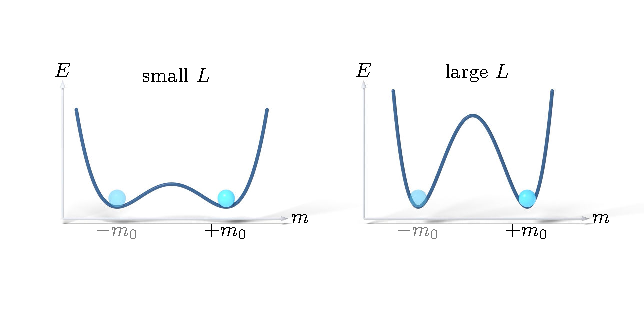
\includegraphics{figures/pdf/s01f02_ssb.pdf}
\end{aqmfigure}
